\documentclass[12pt,a4paper]{article}
%Va a ser un libro (book), el tamaño es a4, la lengua castellano%%%

\usepackage[spanish]{babel} %palabras de multitud de idiomas. Aquí no se si 
\usepackage[utf8]{inputenc} %cambio latin por utf-8
\usepackage{amsmath} %macros AM
\usepackage{amsthm} %macros AMS para teoremas.
\usepackage{amsfonts} %Permite usar fuentes.
%\usepackage[dvips]{epsfig} %Inclusión de figuras postscript
\usepackage{indentfirst}
\usepackage{graphicx}
\graphicspath{{./figs/}}
\usepackage{subfigure}
\usepackage{afterpage}
\usepackage{float}
\newcommand\blankpage{%
	\null
	\thispagestyle{empty}%
	\newpage}
\usepackage{hyperref}
\usepackage{afterpage}
\setlength{\parskip}{8mm} %Separación entre parrafos 
\usepackage{multirow, array} % para las tablas
%\usepackage{longtable} % para tablas largas
\usepackage[left=3 cm,top=2.5cm,right=3cm,bottom=2.5cm]{geometry} 
%\usepackage{cite} % para contraer referencias
\usepackage[utf8]{inputenc}
\usepackage[backend=biber]{biblatex}
\addbibresource{biblio.bib}
\usepackage{setspace}
\usepackage{titlesec}
\spacing{1.5}
\DeclareGraphicsExtensions{.jpg, .pdf, .png, .gif, .eps}
% para nivel 4 de secciones
\setcounter{secnumdepth}{4} 
\setcounter{tocdepth}{4}
\titleformat{\paragraph}
{\normalfont\normalsize\bfseries}{\theparagraph}{1em}{}
\titlespacing*{\paragraph}
{0pt}{3.25ex plus 1ex minus .2ex}{1.5ex plus .2ex}
\usepackage{tabularx}

%% -- encabezado ----
% El encabezado y pie de página forman parte del paquete fancyhdr:
\usepackage{fancyhdr}
\fancyhf{}
\pagestyle{fancy}


% Contenido del encabezado
\rhead{\leftmark}
\renewcommand{\headrulewidth}{0.1pt}


% Contenido del pie de página (\fancyfoot):
\lfoot{\thepage} 
\rfoot{
\includegraphics[width=0.17\textwidth]{logo-eif}}
\renewcommand{\footrulewidth}{0.1pt} 






\begin{document}




%% --------------- PORTADA -----------------------%%

\begin{titlepage}
	
\begin{center}
	\begin{figure}
		\centering
		
\includegraphics[width=0.4\textwidth]{./figs/logoURJC}
	\end{figure}
\end{center}


\begin{center}
	\large
	ESCUELA DE INGENIERÍA DE FUENLABRADA
	\vspace*{0.15in}
\end{center}

\begin{center}
	\large
	GRADO EN INGENIERÍA DE SISTEMAS AUDIOVISUALES Y MULTIMEDIA \\
	\vspace*{0.6in}
\end{center}

\begin{center}
	{\large \bf TRABAJO FIN DE GRADO}\\
\end{center}

\begin{center}
	\vspace*{0.2in}
	{\large
	{PREDICCIÓN DE EMOCIONES A PARTIR DE CARACTERÍSTICAS DE AUDIO MUSICAL UTILIZANDO TÉCNICAS DE APRENDIZAJE MÁQUINA} \\
	}
	\vspace*{0.3in}
	\vspace*{0.3in}
	\vspace*{0.1in}
\end{center}


\begin{center}
	{\large
	Autor: Víctor Iglesias Cuevas  \\[0.2cm]
	Tutora: Rebeca Goya Esteban \\[0.15cm]
	}
	\vspace*{0.1in}
	\vspace*{0.1in}
\end{center}


\begin{center}
	Curso académico 2023/2024\end{center}
\end{titlepage}


%% ------------------- CITA --------------------- %%
\newpage
\thispagestyle{empty} % para que no se numere esta pagina
%\pagenumbering{Roman} % para comenzar la numeracion de paginas en numeros romanos
\begin{flushright}
	\vspace*{5cm}
 	\textit{“Las emociones no son buenas ni malas, son simplemente nuestras respuestas a la vida." (Shari Y. Manning)}
\end{flushright}





%% ------------------- AGRADECIMIENTOS --------------------- %%
\newpage
\thispagestyle{plain}
\addcontentsline{toc}{section}{Agradecimientos}
\section*{Agradecimientos}
 

aquí van los agradecimientos









%% -------------------- RESUMEN --------------------%%
\newpage
\section*{Resumen}
\addcontentsline{toc}{section}{Resumen} % si queremos que aparezca en e
Este Trabajo de Fin de Grado tiene como objetivo desarrollar una aplicación de reconocimiento de emociones en la música (\textit{Music Emotion Recognition, MER}) utilizando técnicas de aprendizaje máquina (\textit{Machine Learning}). La aplicación está diseñada para predecir las emociones musicales a través de las características acústicas de las canciones.


Antes de comenzar con el experimento, se introduce el campo de estudio de MER comentando el marco teórico y su estado actual y futuro, para también poner el foco en las emociones. Para la realización del trabajo es importante conocer qué son las emociones, qué tipos hay, y por qué se ha decidido utilizar para este trabajo las emociones percibidas representadas en un espacio bidimensional formado por valencia y activación.


Una vez asentadas las bases teóricas del trabajo, se da paso a comentar las diferentes técnicas de aprendizaje automático empleadas en el experimento. Se usarán cuatro algoritmos diferentes de \textit{Machine Learning}: árbol de decisión, bosque aleatorio, regresión lineal y regresión \textit{ridge}. Para mejorar la precisión de los modelos de predicción, se han ajustado los hiperparámetros mediante el uso de validación cruzada (\textit{cross-validation}). 


Para elegir los modelos más adecuados para el sistema se han calculado las tasas de error de los algoritmos y se ha elegido la menor de ellas. El resultado del trabajo es un sistema de MER capaz de predecir (con margen de error aceptable para este propuesto) los valores bidimensionales de los que se componen las emociones, y por lo tanto, capaz de predecir las emociones percibidas de las canciones.








%%%%%%%%%%%%%% - INDICE - %%%%%%%%%%%%%
\newpage
\renewcommand*\contentsname{Índice} % Se modifica el nombre por defecto de la "Table Of Contents" (tabla de contenidos, índice) para pasar a llamarla "ÍNDICE".
\tableofcontents
\afterpage{\blankpage} % Se añade una página en blanco después del índice.




%%%%%%%%%%%%%% - INDICE DE TABLAS- %%%%%%%%%%%%%
\newpage
\renewcommand{\listtablename}{Índice de tablas} % Se define el nombre del índice de tablas.
\listoftables % Se genera automáticamente el índice con las distintas tablas del documento (entorno \table o \longtable).
\addcontentsline{toc}{section}{Índice de tablas} % Se añade manualmente el apartado al índice (Table Of Contents, TOC).




%%%%%%%%%%%%%% - INDICE DE FIGURAS- %%%%%%%%%%%%%
\newpage
\renewcommand{\listfigurename}{Índice de figuras} % Se define el nombre del índice de figuras.
\listoffigures % Se genera automáticamente el índice con las distintas figuras del documento (entorno \figure).
\addcontentsline{toc}{section}{Índice de figuras} % Se añade manualmente el apartado al índice (Table Of Contents, TOC).






%%%%%%%%%%%%%% - INTRODUCCIÓN- %%%%%%%%%%%%%
\newpage
%\pagenumbering{arabic} % para empezar la numeración con números
\section{Introducción}
\subsection{Motivación y contexto}
La música juega un rol importante en la vida de la personas, aun más en la era digital. El uso de Internet ha contribuido enormemente en el crecimiento de librerías digitales de música, y con ello, la información y metadatos disponibles de cada pista de audio. El poder emocional de la música es el motivo de su aplicación en áreas tan diversas como la industria del juego, la industria cinematográfica, marketing y musicoterapia, pero los conocimientos científicos sobre este fenómeno están lejos de ser completos o reveladores \cite{eerola2012review}.


La relación entre música y emoción ha sido objeto de muchos debates académicos e investigaciones empíricas en muchas disciplinas diferentes donde están incluidas la filosofía, la musicología, la psicología, la biología, la antropología y la sociología. Sin embargo, no fue hasta la década de los 2000, cuando el estudio de este tema desde el punto de vista de la ingeniería, comenzó a desarrollar un modelo computacional de emoción musical para la recuperación y organización de la música basada en emociones \cite{yang2011music}.


Tradicionalmente, la clasificación de música ha estado basada en catálogos de metadatos (artista, album, título de la canción, ...) \cite{yang2011music}. Esta clasificación puede no ser suficiente para el usuario. Tener acceso a una categorización de la música en función de emociones o estados de ánimo puede ser de gran utilidad para muchas aplicaciones. Imaginemos un reproductor de música que, además de recomendarte canciones según un grupo o un estilo musical, sea capaz de hacerlo según el estado de ánimo que tengas.


Aquí es donde entra en juego el Reconocimiento Musical de Emociones (\textit{Music Emotion Recognition}). MER categoriza emociones y aplica técnicas de \textit{Machine Learning} (Aprendizaje Máquina) para clasificarlas usando diferentes características extraídas de la señal acústica de la canción \cite{yang2011music}.



\subsection{Objetivos del trabajo}
El objetivo principal del trabajo es diseñar un sistema para el reconocimiento de emociones en pistas de audio.
Los objetivos específicos que se plantean son los siguientes:
\begin{itemize}
\item Estudiar el Estado del Arte de los sistemas de MER.
\item Examinar técnicas de Aprendizaje Máquina (\textit{Machine Learning}) para la detección de emociones.
\item Usar lenguage Python para:
 	\begin{itemize}
 		\item procesar datos del banco de datos, 
 		\item desarrollar algoritmos de \textit{Machine Learning},
 		\item entrenar y probar los sistemas para ajustar parámetros,
 		\item evaluar las técnicas de \textit{Machine Learning} según su capacidad para predecir los valores requeridos. 		
 	\end{itemize}
\end{itemize}

\subsection{Metodología y estructura de la memoria}
La memoria está compuesta por cinco apartados:
\begin{enumerate}
	\item Una introducción de la memoria donde se expone el contexto y la motivación del trabajo.
	\item El capítulo de \textit{Estado del arte} donde se expone:
	\begin{itemize}
		\item una introducción al campo de estudio de MER,
		\item una descripción de \textit{Machine Larning} y los diferentes tipos de algoritmos que hay, 
		\item y una explicación de los modelos de regresión y la definición de los usados en el trabajo.
	\end{itemize}
	\item El capítulo de \textit{Experimentos} dividido en:
	\begin{itemize}
		\item descripción de los datos utilizados,
		\item y algoritmos de \textit{Machine Learning} empleados en el trabajo.
	\end{itemize}
	\item Los resultados detallados de los experimentos realizados en el capítulo anterior.
	\item Las conclusiones obtenidas del trabajo, y líneas futuras en las que seguir profundizando en MER.
\end{enumerate}









%%%%%%%%%%%%%% - ESTADO DEL ARTE - %%%%%%%%%%%%%
\newpage
\section{Estado del arte}
\subsection{Music Emotion Recognition}

\textit{Music Emotion Recognition} (MER) es un campo de estudio que se enfoca en identificar y clasificar las emociones que la música evoca en los oyentes. Para ello, se extraen las características relevantes de las pistas de audio, se procesan, se evalúan, y posteriormente se asocian con determinadas emociones \cite{GomezCanon2021SPM}.


MER es una de las disciplinas de alto nivel más desafiantes en \textit{Music Information Retrieval} (MIR). MIR es un campo de investigación que se centra en la extracción y el manejo de características significativas de la música (a partir de la señal acústica), la clasificación de la música utilizando estas características, y el desarrollo de diferentes esquemas de búsqueda y recuperación. Tiene como objetivo poner a disposición de los individuos el vasto almacén de música del mundo \cite{schedl2014music}.

\subsubsection{Emociones}\label{emo}

Los modelos teóricos de la emoción adoptados por los estudios se dividieron en cuatro clases: discretos, dimensionales, misceláneos y específicos de la música \cite{eerola2012review}. 


Uno de los más comunes usado en psicología es el modelo dimensional propuesto por Russell \cite{posner2005circumplex}. El modelo consiste en la representación de las emociones a través de dos dimensiones: valencia (nivel de agrado o desagrado) y activación (representa el nivel de energía o activación de la valencia). Cada emoción es una representación lineal de la combinación de estas dos dimensiones.

\begin{figure}[H]
	\centering
	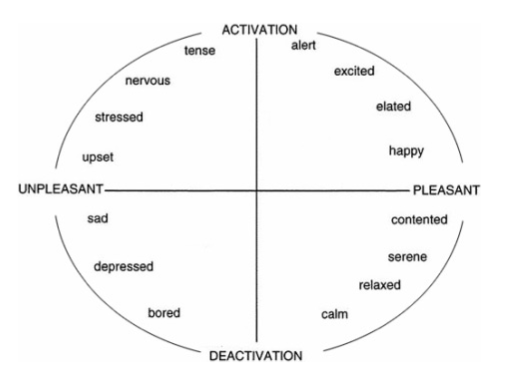
\includegraphics[width=0.7\linewidth]{figs/russell}
	\caption{Modelo dimensional de Russell \cite{posner2005circumplex}}
	\label{fig:russell}
\end{figure}


Un aspecto importante en MER es la categorización de las emociones según su naturaleza. Se distinguen dos tipos:
\begin{itemize}
\item Percibidas: son aquellas que hacen referencia a las características musicales canción: tono, escala, ritmo, etc.
\item Inducidas: son las emociones que hacen referencia al contexto individual de cada persona.
\end{itemize}

\citeauthor{yang2011music} en su libro \citetitle{yang2011music} \cite{yang2011music}, exponen un ejemplo claro para distinguir entre los dos tipos: el Cumpleaños Feliz. Si analizamos la canción por sus características, se podría decir que es una canción alegre (emoción percibida). Pero es posible que para algunas personas les produzca tristeza al asociar un recuerdo con esta canción (emoción inducida).

\subsubsection{Estado actual MER}
El flujo de trabajo en MER se divide en cuatro bloques \cite{GomezCanon2021SPM}:


\paragraph{Taxonomía y propiedades musicales de la emoción}\label{tax_emo}
Es la forma en que se clasifican y categorizan las emociones. Hay dos taxonomías predominantes en el marco actual de MER:
\begin{itemize}
	\item Enfoque categórico/discreto. Presenta diferentes clases: feliz, triste, etc. Este enfoque tiene una resolución mala y resulta ambiguo.
	\item Enfoque dimensional. Como explica el apartado anterior, se conceptualiza la emoción como un elemento bidimensional (valencia y activación). Este enfoque puede resultar más exacto que el anterior, pero también más complejo a la hora de mapear las emociones en el marco que propone Russell \cite{posner2005circumplex}
\end{itemize}

La elección de la taxonomía es la decisión más importante para diseñar un conjunto de datos. Define el nivel de precisión emocional, por lo que su elección marcará el desarrollo del sistema de MER.

\paragraph{Creación del conjunto de datos y recopilación de anotaciones subjetivas}
La forma más utilizada para la recopilación de emociones musicales es la subjetiva. Los anotadores suelen escuchar extractos de canciones (de unos 30 segundos) para posteriormente emitir juicios emocionales. Los datos son anotados siguiendo la taxonomía elegida para la creación del conjunto de datos. Estos anotadores son expertos en música, pero sin conocimiento alguno de teoría musical (musicólogos, productores, investigadores, etc.).


Todas las calificaciones son promediadas para llegar a una ``verdad universal''. Es decir, los valores finales son un promedio de las anotaciones de cada experto.

\paragraph{Extracción de las características}
En los conjuntos de datos se encuentran características de dos tipos: propiedades acústicas a bajo nivel y los niveles musicales a alto nivel. Estos dos tipos de características no tienen por qué estar relacionadas: las propiedades acústicas a bajo nivel se obtienen de la señal acústica de la canción, mientras que los niveles musicales a alto nivel están relacionados con la melodía, ritmo o el tono.


A esta diferencia de características se la denomina ``brecha semántica''. La tendencia actual está enfocada en trabajar para reducir esta brecha: se ha descubierto que el ritmo está relacionado con la estructura métrica y la duración de las notas, o que la dinámica de la canción está relacionada con el volumen, la energía media cuadrática o la intensidad de las notas.


Las herramientas más utilizadas para la extracción de características son:
\begin{itemize}
	\item MIRToolbox. Un conjunto de herramientas en Matlab.
	\item OpenSMILE. Desarrollada en C++.
	\item Essentia 4. Desarrollado en C++, posee clasificadores previamente entrenados.
	\item PsySound. Librería para uso en Matlab basada en algoritmos psicoacústicos.
	\item Librosa. Biblioteca de código abierto para Python. Especializada en el análisis y procesamiento de audio y música. Es ampliamente utilizada en la comunidad de investigación en musicología, así como en aplicaciones prácticas que involucran el procesamiento y análisis de señales de audio en MIR.
\end{itemize}

\paragraph{Evaluación}
La evaluación de los sistemas MER está directamente relacionada con la taxonomía de las emociones: la taxonomía elegida para trabajar en el sistema de MER afecta a las características extraídas y los valores a predecir, y estos a su vez a la evaluación de los sistemas. Hay dos enfoques de sistema de MER:
\begin{itemize}
	\item Sistema de clasificación, si la taxonomía elegida sigue un enfoque categórico/discreto. Los parámetros de evaluación de estos sistemas son los mismos que en modelos de clasificación de otras disciplinas: precisión, f-score, etc.
	\item Sistema de regresión, si el enfoque es dimensional/continuo. Los parámetros comúnmente usados para evaluar estos sistemas son: error cuadrático medio, coeficiente de determinación (R2) o coeficiente de correlación de Pearson ($\rho$).
\end{itemize}
\begin{figure}[H]
	\centering
	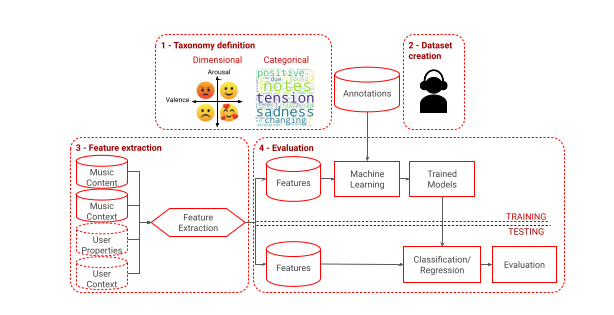
\includegraphics[width=1\linewidth]{figs/mer_traditional_system}
	\caption{Sistema tradicional MER \cite{GomezCanon2021SPM}}
	\label{fig:mertraditionalsystem}
\end{figure}
\subsubsection{Estado futuro MER}
En el libro \citetitle{yang2011music} \cite{yang2011music} se presentan varias vías de trabajo donde MER puede profundizar.

\paragraph{Timbre vocal}
Actualmente, en el análisis emocional de una canción, MER pone el foco en la música y en las letras. Sin embargo, la voz contiene muchos matices que pueden resultar  especialmente valiosos en los modelos de predicción. Los timbres de voz (alegre, rasgado, agudo, agresivo, etc.) afectan a la percepción que tiene el oyente de la canción.


Existen distintas formas de estudiar el timbre vocal basadas en el estudio de la señal acústica de la voz y la extracción de descriptores (\textit{pitch}, energía, coeficientes cepstrum, etc).

\paragraph{Factores de situación}
En el apartado ~\ref{emo} donde se describen las emociones, se hace referencia a las emociones inducidas. La situación del oyente (momento del día, si está acompañado o solo, etc) afecta directamente a las emociones inducidas. El estudio de la situación puede ser de ayuda para dar contexto acerca del entorno que tiene el oyente, y modificar (o no) la predicción de emociones.

\paragraph{Conexión entre enfoques dimensional y categórico}\label{combi}
Como se describe en el apartado ~\ref{tax_emo} hay dos enfoques bien diferenciados en el estudio de MER: dimensional/continuo y categórico/discreto. Una combinación de los dos enfoques puede resultar eficaz.

\subsection{Técnicas de \textit{Machine Learning}}

El \textit{Machine Learning} es la ciencia de programar ordenadores para que estos puedan aprender de los datos \cite{geron2022hands}. Se enfoca en la idea de que los ordenadores puedan ``aprender'' a partir de la experiencia y los datos: identifican patrones en los datos y predicen o deciden en función de esos patrones.

\subsubsection{Tipos de \textit{Machine Learning}}
Los tipos de Machine Learning se clasifican en diferentes categorías según su naturaleza \cite{geron2022hands}:
\begin{itemize}
	\item Grado de supervisión humana durante el entrenamiento. Dentro de esta categoría se encuentran los siguientes sistemas:
	\begin{itemize}
		\item supervisados,
		\item no supervisados,
		\item refuerzo del aprendizaje (\textit{Reinforcement Learning}).
	\end{itemize}
	\item Si pueden o no aprender de forma incremental. Se distinguen dos tipos:
	\begin{itemize}
		\item sistemas en línea (\textit{Batch Learning}),
		\item sistemas por lotes (\textit{Online Learning}).
	\end{itemize}
	\item Si detectan o no patrones en los datos de entrenamiento, construyendo un modelo predictivo. Tipos:
	\begin{itemize}
		\item basados en instancias,
		\item basados en modelos.
	\end{itemize}
\end{itemize}

Estos criterios no son exclusivos. Pueden combinarse de la forma que se quiera.

\subsubsection{Sistemas supervisados vs. no supervisados}
Los sistemas supervisados de \textit{Machine Learning} son algoritmos que utilizan datos etiquetados (etiquetas) durante la fase de entrenamiento del sistema. Son utilizados tanto para modelos de clasificación como para modelos de regresión (predicción de un número dado un paquete de características). Algunos de los algoritmos supervisados más importantes son:
\begin{itemize}
	\item KNN 
	\item Regresión lineal
	\item Regresión logística
	\item Redes Neuronales	
\end{itemize}

Por otro lado nos encontramos los sistemas no supervisados. Se utilizan para encontrar patrones o estructuras ocultas en datos. A diferencia de los supervisados, estos algoritmos no utilizan ningún etiquetado ni requieren de ninguna salida deseada durante el entrenamiento. Tipos de algoritmos no supervisados:
\begin{itemize}
	\item Agrupamiento (\textit{Clustering})
	\begin{itemize}
		\item K-medias
		\item DBSCAN
		\item Análisis de agrupamiento jerárquico (HCA)	
	\end{itemize}
	\item Detección de anomalías
	\begin{itemize}
		\item \textit{One-class SVM}
		\item \textit{Isolation Forest}	
	\end{itemize}
	\item Reducción de dimensionalidad
	\begin{itemize}
		\item Análisis de componentes principales (PCA)
		\item \textit{Kernel PCA}	
		\item \textit{Locally-Linear Embedding} (\textit{LLE})
		\item \textit{t-distributed Stochastic Neighbor Embedding} (\textit{t-SNE})
	\end{itemize}
	\item Aprendizaje de reglas de asociación
	\begin{itemize}
		\item Apriori
		\item Eclat	
	\end{itemize}	
\end{itemize}

\subsubsection{\textit{Batch Learning} y \textit{Online Learning}}
Los sistemas \textit{Batch Learning} son incapaces de aprender de forma incremental. El modelo se entrena utilizando la totalidad del conjunto de datos de entrenamiento de una sola vez, en lugar de hacerlo de manera incremental o en pequeñas partes. Dada la forma de entrenar, estos sistemas son capaces de captar mejor las complejidades y las variabilidades de los datos. Sin embargo, son más vulnerables frente a cambios en los datos puesto que sería necesario volver a entrenar el modelo de nuevo.


Los sistemas \textit{Online Learning} son lo contrario a los anteriores: se entrenan de forma incremental. Se dividen los datos en pequeñas instancias (o \textit{mini-batches}) y se alimenta el sistema de forma secuencial. Cada aprendizaje es rápido y barato. Se utiliza para sistemas donde se reciben datos de forma continua, o cuando no se requiere una gran cantidad de datos para el entrenamiento. En estos modelos es importante el parámetro de tasa de aprendizaje (\textit{learning rate}): una tasa de aprendizaje alta hará que el sistema se adapte bien a cambios en los datos, pero también será más susceptible a olvidar más rápido datos antiguos.


\subsubsection{Basados en instancias y Basados en modelos}
Esta clasificación hace referencia a cómo los sistemas de \textit{Machine Learning} se generalizan. Por un lado están los basados en instancias: el sistema aprende los ejemplos de memoria y luego generaliza a nuevos casos comparándolos con los ejemplos aprendidos (o un subconjunto de
ellos). Es decir, utiliza una medida de similitud. Estos sistemas tiene un buen rendimiento con datos entrenados, pero no es suficiente para un sistema de \textit{Machine Learning}: el verdadero objetivo es tener un buen rendimiento en instancias nuevas.


Aquí es donde se encuentran los sistemas basados en modelos, cuya forma de generalizar es a partir de modelos que hagan predicciones. Estos sistemas tienen mucho mejor rendimiento frente a instancias de datos muy ruidosas (gran cantidad de datos aleatorios). Para conseguir buenos resultados con estos sistemas se deben seguir algunos pasos como: selección del modelo (elegir el mejor modelo que se adapte a nuestro sistema), ajuste del modelo (elección correcta de los parámetro o hiperparámetros),  o entrenamiento del modelo.

\subsubsection{Validación cruzada}\label{cross-validation}
La validación cruzada (o \textit{cross-validation}) es una técnica fundamental para la evaluación y selección de modelos en el contexto del aprendizaje estadístico. Se utiliza para evaluar la capacidad predictiva de un modelo, permitiendo estimar cómo de bien funcionará el modelo en datos no vistos. Este procedimiento es crucial para evitar el sobreajuste (\textit{overfitting}) y para comparar de manera objetiva el rendimiento de diferentes modelos o ajustes de hiperparámetros.


Para entender mejor esta técnica, se parte de la diferencia entre la tasa de error de test y la tasa de error de entrenamiento. La tasa de error de test se calcula fácilmente comparando los datos obtenidos en la predicción (se introducen en el modelo entrenado las variables independientes, para obtener la predicción de la variable objetivo) con los datos reales. Sin embargo, la tasa de error de entrenamiento no se puede calcular (sin emplear una técnica precisa para ello), al ser el mismo conjunto de datos (datos de entrenamiento) que usaríamos para entrenar y validar \cite{gareth2013introduction}.


Existen diferentes tipos de \textit{cross-validation}, pero el más utilizado es \textit{K-Fold}. Parte de la idea de dividir el conjunto de datos de entrenamiento en \textit{k} particiones (ver Figura \ref{fig:cross-validation}), de las cuales se usarán \textit{k-1} para entrenamiento y la restante para la validación. Este proceso se repite de forma iterativa, de manera que todas las particiones se han usado una vez para validar y \textit{k-1} veces para entrenar \cite{hastie2009elements}.
\begin{figure}[H]
	\centering
	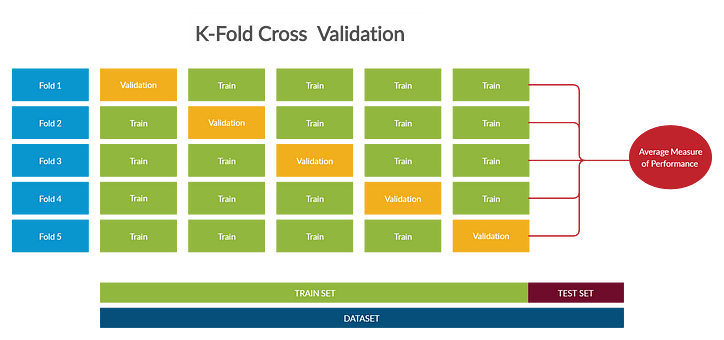
\includegraphics[width=0.7\linewidth]{figs/cross-validation}
	\caption{Ejemplo de funcionamiento de \textit{cross-validation} para $k = 5$ \cite{crossvalidation}}
	\label{fig:cross-validation}
\end{figure}
En cada iteración se calculan las métricas de rendimiento, para finalmente, hacer un promedio y obtener una estimación total del rendimiento del modelo.
A pesar de que esta técnica puede resultar computacionalmente intensiva, proporciona una estimación más fiable del modelo utilizando todos los datos de entrenamiento de una forma más eficiente.



\subsection{Modelos de regresión}
Los modelos de regresión son técnicas que se utilizan para predecir un valor numérico continuo basado en una o más variables independientes. Para ello, se modela el efecto de un conjunto de variables explicativas sobre una varibale de interés primario \autocite{fahrmeir2013regression}.


Los conceptos fundamentales de los modelos de regresión son:
\begin{itemize}
	\item Variable dependiente (variable objetivo, respuesta o de interés primario): es la variable que se desea predecir. Esta puede ser continua, binaria, categórica o de recuentos.
	\item Variables explicativas: también llamadas covariables, variables independientes o regresoras. Son las que se utilizan para predecir la variable dependiente. Existen varios tipos de estas variables como continuas, binarias, o categóricas. En modelos complejos también es posible incluir escalas temporales, variables para describir la distribución espacial o la ubicación geográfica, o indicadores grupales.
	\item Tipo de modelo: dependerá principalmente del tipo de variable respuesta, y del tipo de variables independientes.
\end{itemize}

Una característica principal de los modelos de regresión es que la relación entre la variable objetivo y las variables independientes no es una función determinista, si no que muestra errores. Esto implica que la respuesta \textit{y} es una variable aleatoria, cuya distribución depende de las variables independientes. Un ejemplo claro sería: sabiendo la altura de los padres no se puede predecir exactamente la altura de los hijos, solo estimar una media y el grado de dispersión. A esta desviación del valor esperado se la denomina $\epsilon$ (componente aleatorio o estocástico). Por eso es muy importante estudiar la importancia de las covariables en el valor medio de la variable objetivo. La función resultante es un modelo condicional donde los valores de \textit{y} (variable objetivo) están condicionados por las covariables ($x_1, x_2, x_3, ...$) y el componente aleatorio $\epsilon$:

\begin{equation}
	y = E(y|x_1, ..., x_k) = f(x_1, ..., x_k) + \epsilon 
\end{equation}


\subsubsection{Árboles de decisión}\label{decision_tree}
Los árboles de decisión son una técnica de \textit{Machine Learning} y estadística utilizada tanto para casos de clasificación como para casos de regresión. Son modelos predictivos que representan decisiones y sus posibles consecuencias, incluidas las probabilidades de diferentes resultados. Son conceptualmente simples, pero poderosos.


El principio de los árboles de regresión es segmentar el espacio de las características en una serie de regiones simples. El conjunto de reglas de división utilizadas para segmentar el espacio se pueden resumir en un árbol, de ahí el término \cite{gareth2013introduction}.


En el libro \citetitle{hastie2009elements} \cite{hastie2009elements} se explican los modelos de decisión con un ejemplo simple: imaginemos un problema de regresión con una respuesta continua $Y$ y los \textit{inputs} $X_1$ y $X_2$. Primero se divide el espacio en dos regiones. Se elige la variable y el punto de división para lograr el mejor ajuste. Luego, una o ambas regiones se dividen en dos regiones más. El proceso continua hasta que se aplica alguna regla de detención.



\begin{figure}[H]
	\centering
	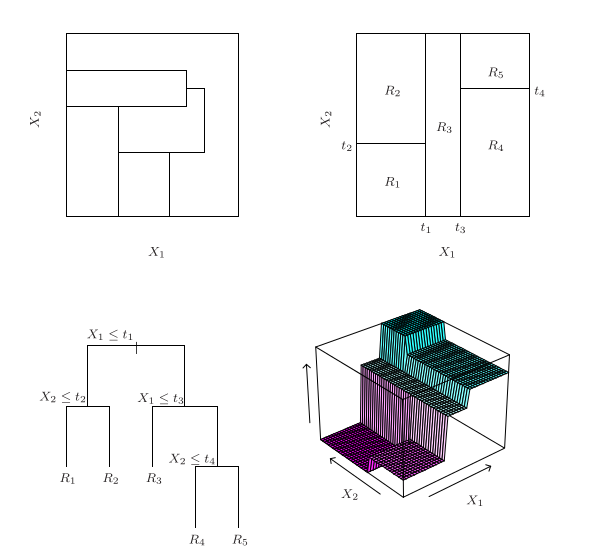
\includegraphics[width=0.7\linewidth]{figs/decission_tree}
	\caption{Funcionamiento de un árbol de decisión \cite{gareth2013introduction}}
	\label{fig:decissiontree}
\end{figure}


Los métodos basados en árboles de decisión son simples, y útiles para la interpretación. Sin embargo, normalmente no son competitivos con los mejores enfoques de aprendizaje supervisado en términos de predicción \cite{gareth2013introduction}.

\subsubsection{Bosque aleatorio}
Bosque aleatorio (\textit{random forests}) es un método de aprendizaje para clasificación y regresión que consiste en construir una multitud de árboles de decisión (ver ~\ref{decision_tree}) en la etapa de entrenamiento, y así obtener el modo de las clases (clasificación) o la media de las predicciones (regresión) de los árboles individuales.


La idea de los bosques aleatorios es reducir la varianza del sistema, reduciendo la correlación entre los árboles (sin incrementar en exceso la varianza). Esto es posible gracias a una selección aleatoria de variables independientes durante el proceso de crecimiento de los árboles \cite{hastie2009elements}.


La forma en que se construye los bosques aleatorios es la siguiente:
\begin{enumerate}
	\item Se elige el número $B$ de árboles de decisión que formará el bosque.
	\item Se hace crecer los árboles del bosque repitiendo de forma recursiva los siguientes pasos:
	\begin{enumerate}
		\item Del conjunto de datos de entrenamiento, se elige un subconjunto aleatorio de las características (generalmente $\sqrt{\rho}$ variables si hay $\rho$ en total).
		\item De este subconjunto, se elige la mejor variable.
		\item Se dividen los nodos en dos nodos hijos.
	\end{enumerate}
	\item Se obtienen los datos del conjunto de árboles.
	\item Se hace la predicción.
\end{enumerate}


\subsubsection{Regresión lineal}
La regresión lineal es uno de los métodos más básicos y  utilizados de regresión. Como se explica en el apartado anterior, en regresión existe una relación entre la variable objetivo y las variables independientes a través de la función $f(x_1, ..., x_k)$. Esta función no es exacta al estar afectada por el ruido $\epsilon$. El objetivo es estimar la función desconocida $f$, es decir, separar el componente sistemático de $f$ del ruido aleatorio $\epsilon$, asumiendo en este caso un acercamiento lineal \cite{fahrmeir2013regression}. La ecuación resultante es la siguiente:
\begin{equation}
	y_i = 
	\beta_0 + \beta_1x_i, ..., \beta_kx_i + \epsilon_i = 
	 x'_i\beta + \epsilon 
\end{equation}
 
Donde los parámetros $\beta_0, \beta_1, ..., \beta_k$ son desconocidos y deben ser estimados. El parámetro $\beta_0$ representa la intersección (cuando el valor de $x$ es 0).

\begin{figure}[H]
	\centering
	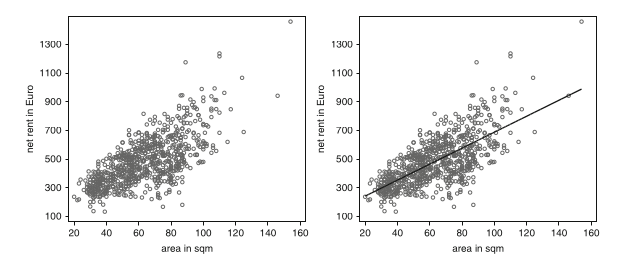
\includegraphics[width=0.7\linewidth]{figs/linear_regression}
	\caption{Regresión lineal \cite{fahrmeir2013regression}}
	\label{fig:linearregression}
\end{figure}
El objetivo de la regresión lineal es encontrar la mejor línea recta que minimice la suma de los errores cuadrados (diferencias entre los valores reales y los valores predichos).

\subsubsection{Regresión \textit{ridge}}
La regresión \textit{ridge} es una variante de la regresión lineal estándar. Modifica la estimación de los coeficientes del modelo para mejorar la precisión: introduce una penalización que reduce los coeficientes de las variables independientes. Para lograr esta penalización se agrega un término de regulación que es proporcional a la suma de los cuadrados de los coeficientes. La fórmula de la regresión \textit{ridge} es la siguiente \cite{hastie2009elements}:
\begin{equation}
	\hat{\beta}^{ridge} = argmin {\sum_{i=1}^{N}} (y_i - \beta_0 - \sum_{k=1}^{p}x_{ik}\beta^{2}_k)
\end{equation}

Donde:
\begin{itemize}
	\item $\hat{\beta}^{ridge}$ es el término de regularización \textit{ridge},
	\item $y_i$ es la variable respuesta para la observación $i$,
	\item $N$ es el número de observaciones,
	\item $x_{ik}$ es el valor de la variable independiente $k$ para la observación $i$,
	\item $\beta_{k}$ son los coeficientes del modelo,
	\item $p$ es el número de coeficientes de la observación.
\end{itemize}

La regresión \textit{ridge} se utiliza cuando hay muchas variables independientes y se quiere mejorar la precisión del modelo lineal: los coeficientes puede estar mal determinados y mostrar una varianza muy alta. Al imponer una restricción de tamaño de los coeficientes se soluciona este problema \cite{fahrmeir2013regression}.










%%%%%%%%%%%%%% - EXPERIMENTOS - %%%%%%%%%%%%%
\newpage
\section{Experimentos}
En este capítulo se describe el proceso del desarrollo de la aplicación de MER. Primero, se describe el conjunto de datos utilizado en el experimento, y cómo los datos han sido manipulados para ser empleados por el sistema. Por último, se describen las técnicas de \textit{Machine Learning} utilizadas en la aplicación.


\subsection{Conjunto de datos}
El conjunto de datos elegido para el experimento es \textit{DEAM dataset - The MediaEval Database for Emotional Analysis of Music} \cite{AlajankiEmoInMusicAnalysis}. El conjunto de datos DEAM consta de 1802 extractos y canciones libres de derechos que provienen de varias fuentes: freemusicarchive.org (FMA), jamendo.com,
y el conjunto de datos medleyDB.


Existen tres tipos de información claramente diferenciables por cada pista de audio del conjunto de datos: características, valores de valencia y activación, y metadatos.

\subsubsection{Características}
Los datos presentan un conjunto de características extraídas de la librería \textit{openSMILE} \cite{openSMILE}. Cada pista de audio está representada en un fichero CSV, donde las pistas se dividen en ventanas de 500ms. En cada ventana se muestran dos valores de cada una de las características: la media y la desviación estándar. Las características presentes en el conjunto de datos son \cite{openSMILEfeatures}:
\begin{itemize}
	\item Energía.
	\item Intensidad de fotograma (energía de un segmento corto de la señal de audio).
	\item Coeficientes cepstrales Mel (MFCC) y coeficientes cepstrales Bark. Las escalas Mel y Bark son escalas perceptuales de frecuencias que aproximan a la forma en que los humanos perciben los sonidos. Se calculan los coeficientes de estas escalas para parametrizar las pistas de audio de forma que se refleje la percepción humana.
	\item Espectros de banda crítica (Mel/Bark/Octave y filtros de enmascaramiento triangulares).
	\item Espectros auditivos.
	\item Sonoridad (medida de cómo los humanos perciben la intensidad de los sonidos) aproximada a partir de espectros auditivos.
	\item Coeficientes predictivos lineales (LPC). Estos parámetros representan la señal de audio como la salida de un filtro lineal predictivo.
	\item Coeficientes perceptivos lineales predictivos (PLP): similares a los LPC, pero incorporando aspectos perceptuales basados en la audición humana.
	\item Coeficientes cepstrales predictivos lineales perceptivos (PLP-CC). Son iguales que los anteriores pero combinados con la representación cepstral.
	\item Pares espectrales de líneas (LSP) que representan frecuencias resonantes de la señal de audio.
	\item Frecuencia fundamental obtenida mediante la función de autocorrelación (ACF) y mediante sumación subarmónica SHS (suma de los armónicos de la señal).
	\item Probabilidad de emisión de voz a partir del pico del espectro ACF y SHS.
	\item Calidad de voz mediante el \textit{Jitter} y el \textit{Shimmer}. El \textit{Jitter} mide la variabilidad temporal de la señal de audio, mientras que el \textit{Shimmer} mide la variabilidad de la amplitud.
	\item Frecuencias de formantes y anchos de banda.
	\item Tasa de cruce por cero y media.
	\item Características espectrales como la energía de bandas arbitrarias, puntos de caída, centroide, entropía, máximos, mínimos, varianza, asimetría, curtosis (concentración pronunciada de energía en torno a ciertas frecuencias) o pendiente.
	\item Armonía espectral (presencia de componentes armónicos) para representar la nitidez psicoacústica.
	\item CROMA, para representar la distribución de energía espectral en semitonos. Y funciones CENS (CROMA suavizado) para obtener una representación suavizada y robusta de las características tonales de la señal.
	\item Funciones derivadas de CROMA para reconocimiento de acordes.
	\item Relaciones de armónicos.
\end{itemize}

\subsubsection{Valencia y activación}
Los datos de valencia y activación se muestran en el conjunto de datos como valores continuos dentro del rango [1, 9].


Para la extracción de estos valores, se eligieron 45 segundos de cada canción de forma aleatoria (posteriormente se descartaron los 15 primeros segundos debido a la inestabilidad de las anotaciones al inicio de los clips). Los 45 segundos se dividieron en ventanas de 500ms, y por cada ventana se anotaron 10 valores para de valencia y activación.


En el conjunto de datos están presentes todas estas anotaciones, junto con los valores de media y desviación estándar de cada canción. Serán estos últimos lo que se usarán en el desarrollo del trabajo.



\subsubsection{Metadatos}
En el conjunto de datos de DEAM \cite{AlajankiEmoInMusicAnalysis} también hay información acerca de las canciones: título de la canción, artista, álbum, géneros musicales y etiquetas.




\subsection{Desarrollo}
En este apartado se describen los pasos a seguir en el desarrollo del sistema de MER. El sistema está compuesto, en primer lugar, por un procesado de datos: se toman los archivos proporcionados por el conjunto de datos y se manipulan para crear las variables de las que están formados los modelos.


Por último, se documenta todo el desarrollo seguido para el diseño de la aplicación. En los siguientes apartados se procede a explicar cómo se han diseñado y entrenado los modelos  para cada uno de los algoritmos. Los algoritmos de \textit{Machine Learning} elegidos son:
\begin{itemize}
	\item Árbol de decisión
	\item Bosque aleatorio
	\item Regresión lineal
	\item Regresión \textit{ridge}
\end{itemize}

La taxonomía elegida para este experimento es la continua/dimensional (ver apartado ~\ref{tax_emo}), donde las emociones están representadas por dos valores: valencia y activación. Visto desde el punto de vista de \textit{Machine Learning}, se presenta un sistema de predicción donde hay dos variables objetivo. Por lo tanto, es necesario dividir el problema en dos sistemas diferentes. El resultado son dos modelos de predicción diferentes para cada algoritmo (uno para valencia y otro para activación).


Tanto la memoria como el código están disponibles en este repositorio Github \url{https://github.com/viglescue/tfg}. El código fuente de la aplicación de MER está dividido en dos archivos: \textit{data-recap.ipynb} con todo el desarrollo correspondiente al procesamiento de datos y archivos del conjunto de datos, y \textit{MER-ML-models.ipynb} con el desarrollo de los diferentes algoritmos para la predicción de emociones. El experimento al completo está desarrollado en lenguaje Python, utilizando cuadernos Jupyter en el entorno de Anaconda. 







\subsubsection{Extracción y manipulación de los datos}
El conjunto de datos DEAM \cite{AlajankiEmoInMusicAnalysis} organiza los datos de la siguiente forma:
\begin{itemize}
	\item Documentos CSV (uno por cada pista de audio) con los valores de las características para cada canción. En cada documento CSV aparece el valor de cada característica en intervalos de 500ms.
	\item Un archivo CSV con los valores de media y desviación para valencia y activación.
\end{itemize}

La idea es recopilar todos los datos en una tabla para manipularlos mejor. Para ello se ha empleado la librería Pandas \cite{mckinney-proc-scipy-2010} para su uso en lenguaje Python.


Para empezar a construir la tabla, primeramente, se obtienen los nombres de las características a partir de uno de los archivos CSV que las contienen. Dado que los valores de características están disponibles por intervalos de 500ms, se ha calculado la media de los valores de cada característica (por cada pista de audio) con el fin de obtener un solo valor por característica y canción. Estos valores serán las variables independientes que se usarán posteriormente en los modelos de ML.


De otro archivo, se han recopilado los valores de media y activación de cada pista de audio. Estos serán las variables dependientes (o variables objetivo) de los modelos.


El resultado es el documento \textit{recap-data.csv}, el cual contiene todas las variables necesarias para construir los modelos de ML.

\begin{figure}[H]
	\centering
	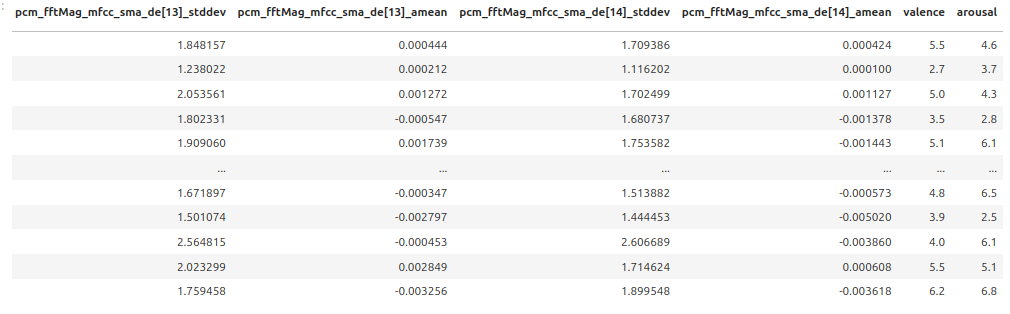
\includegraphics[width=1\linewidth]{figs/data}
	\caption{Recopilación de datos}
	\label{fig:data}
\end{figure}
Una vez recopilados los datos en la tabla que se muestra en la Figura \ref{fig:data}, se definen las variables independientes y las variables objetivo del sistema. Como se comenta en el apartado anterior, esta aplicación de MER se compone de dos variables objetivo. Por lo tanto, las variables se dividen en: un conjunto de variables independientes, una variable objetivo para la valencia, y otra variable objetivo para la activación.
\begin{figure}[H]
	\centering
	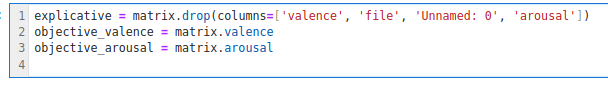
\includegraphics[width=0.8\linewidth]{figs/variables}
	\caption{Definición de variables explicativas y variables objetivo}
	\label{fig:variables}
\end{figure}
Un último procesado de datos antes de empezar con el diseño de los modelos es la división del conjunto de datos entre datos de entrenamiento y datos de test. Para ello se ha utilizado la función \textit{train\_test\_split} de la librería \textit{scikit-learn} de Python \cite{scikit-learn}. Esta función permite la división de datos de forma aleatoria para que haya todo tipo de datos tanto en el conjunto de entrenamiento como en el de test. Los porcentajes elegidos para este trabajo son: 90\% para el conjunto de datos para entrenamiento, y 10\% para test.


En resumen, los sistemas quedan definidos de la siguiente forma:
\begin{itemize}
	\item Sistema para la predicción de valencia (Figura \ref{fig:splitvalence}):
	\begin{itemize}
		\item Variables de entrenamiento: \textit{X\_train\_va}l, \textit{y\_train\_val}
		\item Variables de test: \textit{X\_test\_val}, \textit{y\_test\_val}
		\item Porcentaje de datos de entrenamiento: 90,
		\item Porcentaje de datos de entrenamiento: 10.
	\end{itemize}
	\item Sistema para la predicción de activación (Figura \ref{fig:splitarousal}):
	\begin{itemize}
		\item Variables de entrenamiento: \textit{X\_train\_ar}, \textit{y\_train\_ar}
		\item Variables de test: \textit{X\_test\_ar}, \textit{y\_test\_ar}
		\item Porcentaje de datos de entrenamiento: 90,
		\item Porcentaje de datos de entrenamiento: 10.
	\end{itemize}

\end{itemize}

\begin{figure}[H]
	\centering
	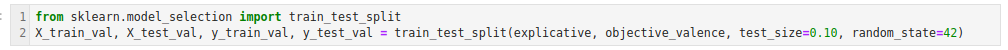
\includegraphics[width=1\linewidth]{figs/split_valence}
	\caption{Definición de variables para valencia}
	\label{fig:splitvalence}
\end{figure}
\begin{figure}[H]
	\centering
	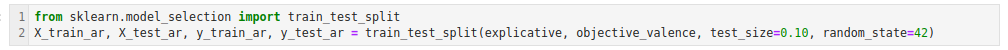
\includegraphics[width=1\linewidth]{figs/split_arousal}
	\caption{Definición de variables para activación}
	\label{fig:splitarousal}
\end{figure}




\subsubsection{Validación cruzada y \textit{GridSearchCV}}\label{gridsearchcv}
En el apartado ~\ref{cross-validation} se describe el concepto de \textit{cross-validation} y su importancia en el diseño de un modelo de \textit{Machine Learning}. En este experimento se ha implementado \textit{cross-validation} mediante el uso de la función \textit{GridSearchCV} de la librería \textit{scikit-learn} de Python \cite{scikit-learn} en todos los modelos. Se ha utilizado esta técnica para encontrar la mejor combinación de hiperparámetros en los modelos.


\textit{GridSearchCV} obtiene como entrada un espacio de valores para cada parámetro del modelo, para posteriormente, evaluar todas las combinaciones de valores posibles. La salida de la función será el valor de cada parámetro del modelo que tenga mejor precisión (\textit{score}).


Los parámetros de entrada para \textit{GridSearchCV} son:
\begin{itemize}
	\item \textit{estimator}: algoritmo de \textit{Machine Learning} utilizado.
	\item \textit{param\_grid}: espacio de valores para los parámetros del algoritmo.
	\item \textit{scoring}: estrategia para evaluar el desempeño del modelo.
	\item \textit{n\_jobs}: número de trabajos que se ejecutarán en paralelo.
	\item \textit{refit}: reajuste del estimador.
	\item \textit{cv}: divisiones para la validación cruzada (\textit{k-folds}, ver ~\ref{cross-validation}).
	\item \textit{verbose}: controla los mensajes de salida.
	\item \textit{pre\_dispatch}: controla el consumo de CPU.
	\item \textit{error\_score}: valor a asignar a la puntuación si se produce un error en el ajuste del estimador.
	\item \textit{return\_train\_score}: si se incluyen o no las puntuaciones de entrenamiento.
\end{itemize}

Los parámetros de entrada para \textit{GridSearchCV} se han configurado como:
\begin{itemize}
	\item \textit{estimator}: la función de \textit{scikit-learn} correspondiente al modelo que se usa.
	\item \textit{param grid}: la variable definida previamente con el espacio de datos para cada modelo.
	\item \textit{scoring}: \textit{None} (valor por defecto).
	\item \textit{n\_jobs}: valor '-1', para utilizar todo el procesador.
	\item \textit{refit}: '\textit{True}' (valor por defecto).
	\item \textit{cv}: 5 \textit{k-folds}. Cinco particiones es lo más común para \textit{cross-validation}.
	\item \textit{verbose}: '10', para obtener toda la información.
	\item \textit{pre\_dispatch}: '\textit{2*n\_jobs}' (valor por defecto).
	\item \textit{error\_score}: 'np.nan' (valor por defecto).
	\item \textit{return\_train\_score}: '\textit{Falso}' (valor por defecto).
\end{itemize}
\begin{figure}[H]
	\centering
	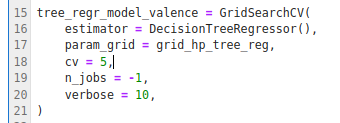
\includegraphics[width=0.7\linewidth]{figs/cv_tree}
	\caption{Ejemplo de configuración de \textit{GridSearchCV} para árbol de decisión}
	\label{fig:cvtree}
\end{figure}



\subsubsection{Árbol de decisión}
Para la creación del árbol de decisión, se ha utilizado la función \textit{DecisionTreeRegressor} del módulo \textit{tree}, perteneciente a la librería \textit{scikit-learn} de Python \cite{scikit-learn}.


El ajuste de hiperparámetros del modelo se ha realizado mediante una validación cruzada exhaustiva utilizando \textit{GridSearchCV} (ver apartado ~\ref{gridsearchcv}). Esta función está presente en el módulo \textit{model\_selection} de \textit{sckit-learn} \cite{scikit-learn}).
\begin{figure}[H]
	\centering
	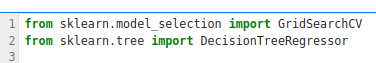
\includegraphics[width=0.7\linewidth]{figs/import_tree}
	\caption{Uso de las funciones \textit{DecisionTreeRegressor} y \textit{GridSearchCV} de \textit{sckit-learn}}
	\label{fig:importtree}
\end{figure}

Mediante la variable \textit{grid\_hp\_tree\_reg} mostrada en la Figura \ref{fig:paramstree} se ha definido un espacio de valores de condiguración del árbol de decisión. Esta variable será el valor de entrada del parámetro \textit{param\_grid} en el proceso de validación cruzada exhaustiva de \textit{GridSearchCV}.
\begin{figure}[H]
	\centering
	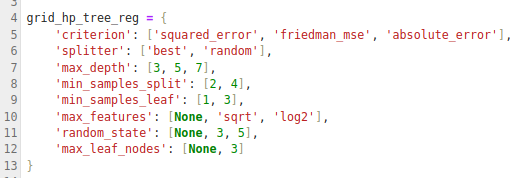
\includegraphics[width=0.7\linewidth]{figs/params_tree}
	\caption{Variable \textit{grid\_hp\_tree\_reg} para la validación cruzada de \textit{DecisionTreeRegressor}}
	\label{fig:paramstree}
\end{figure}

La validación cruzada da como resultado la siguiente combinación de hiperparámetros para el árbol de decisión, la más precisa dentro del espacio de valores de los parámetros contenidos en \textit{grid\_hp\_tree\_reg}:
\begin{itemize}
	\item Para valencia:
	\begin{figure}[H]
		\centering
		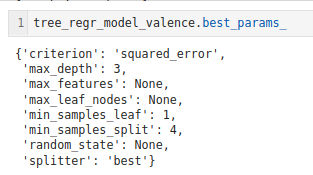
\includegraphics[width=0.5\linewidth]{figs/final_params_tree}
		\caption{Hiperparámetros del árbol de decisión para la predicción de valencia}
		\label{fig:finalparamstree}
	\end{figure}
	\item Para activación:
	\begin{figure}[H]
		\centering
		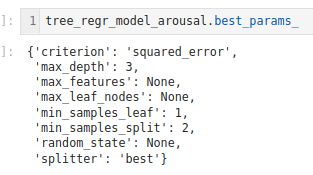
\includegraphics[width=0.5\linewidth]{figs/final_params_tree_arousal}
		\caption{Hiperparámetros del árbol de decisión para la predicción de activación}
		\label{fig:finalparamstreearousal}
	\end{figure}
\end{itemize}

Una vez obtenidos los hiperparámetros se construye el algoritmo de árbol de decisión. Después se entrena el modelo con las variables de entrenamiento (\textit{X\_train\_val} y \textit{y\_train\_val} para valencia, y \textit{X\_train\_ar} y \textit{y\_train\_ar} para activación).


En este punto del experimento, el árbol de decisión está listo para ser utilizado con los datos de test (\textit{X\_test \_val} y \textit{X\_test\_ar}). La precisión y la fiabilidad del modelo será evaluada en el capítulo \ref{resultados}.

\subsubsection{Bosque aleatorio}
Para la creación de bosques aleatorios, se ha utilizado la función \textit{RandomForestRegressor} del módulo \textit{ensemble}, perteneciente a la librería \textit{scikit-learn} de Python \cite{scikit-learn}.


El ajuste de hiperparámetros del modelo se ha realizado mediante una validación cruzada exhaustiva utilizando \textit{GridSearchCV} (función presente en el módulo \textit{model\_selection} de \textit{sckit-learn} \cite{scikit-learn}).

Para este modelo, los valores de entrada de la variable \textit{param\_grid} de \textit{GridSearchCV} están contenidos en la la variable \textit{grid\_hp\_random\_forest} (ver Figura \ref{fig:paramsforest}).
\begin{figure}[H]
	\centering
	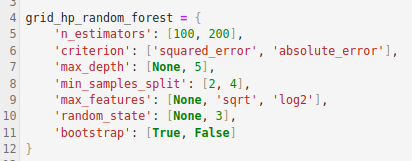
\includegraphics[width=0.7\linewidth]{figs/params_forest}
	\caption{Variable \textit{grid\_hp\_random\_forest} para la validación cruzada de \textit{LinearRegression}}
	\label{fig:paramsforest}
\end{figure}


La validación cruzada da como resultado los hiperparámetros:
\begin{itemize}
	\item Para valencia:
	\begin{figure}[H]
		\centering
		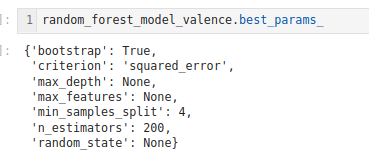
\includegraphics[width=0.7\linewidth]{figs/final_params_random_forest_valence}
		\caption{Hiperparámetros del bosque aleatorio para la predicción de valencia}
		\label{fig:finalparamsrandomforestvalence}
	\end{figure}
	\item Para activación:
	\begin{figure}[H]
		\centering
		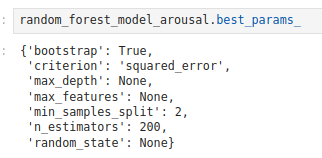
\includegraphics[width=0.7\linewidth]{figs/final_params_random_forest_arousal}
		\caption{Hiperparámetros del bosque aleatorio para la predicción de activación}
		\label{fig:finalparamsrandomforestarousal}
	\end{figure}
\end{itemize}

Una vez obtenidos los hiperparámetros se construye el algoritmo de bosque aleatorio. Posteriormente, se entrena el modelo con las variables de entrenamiento (\textit{X\_train\_val} y \textit{y\_train\_val} para valencia, y \textit{X\_train\_ar} y \textit{y\_train\_ar} para activación).


En este punto del experimento, el bosque aleatorio está listo para ser utilizado con los datos de test (\textit{X\_test\_val} y \textit{X\_test\_ar}). La precisión y la fiabilidad del modelo será evaluada en el capítulo \ref{resultados}.

\subsubsection{Regresión Lineal}
Para la implementación de los modelos de regresión lineal, se ha utilizado la función \textit{LinearRegression} del módulo \textit{linear model}, perteneciente a la librería \textit{scikit-learn} de Python \cite{scikit-learn}.


Para el ajuste de hiperparámetros del modelo, se ha utilizado \textit{GridSearchCV} (función presente en el módulo \textit{model selection} de \textit{sckit-learn} \cite{scikit-learn}) para realizar una validación cruzada exhaustiva.
\begin{figure}[H]
	\centering
	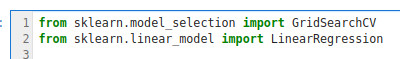
\includegraphics[width=0.7\linewidth]{figs/import_linear_reg}
	\caption{Uso de las funciones \textit{LinearRegression} y \textit{GridSearchCV} de \textit{sckit-learn}}
	\label{fig:importlinearreg}
\end{figure}
Mediante la variable \textit{grid\_hp\_linear\_reg} mostrada en la Figura \ref{fig:paramslinearreg} se ha definido un espacio de valores de configuración del árbol de decisión. Esta variable será el valor de entrada del parámetro \textit{param\_grid} en el proceso de validación cruzada exhaustiva de \textit{GridSearchCV}.
\begin{figure}[H]
	\centering
	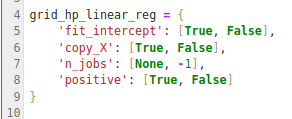
\includegraphics[width=0.7\linewidth]{figs/params_linear_reg}
	\caption{Variable \textit{grid\_hp\_linear\_reg} para la validación cruzada de \textit{LinearRegression}}
	\label{fig:paramslinearreg}
\end{figure}
La validación cruzada da como resultado la combinación de parámetros de entrada donde la función \textit{LinearRegression} tiene una mayor precisión. Los hiperparámetros obtenidos son:
\begin{itemize}
	\item Para valencia:
	\begin{figure}[H]
		\centering
		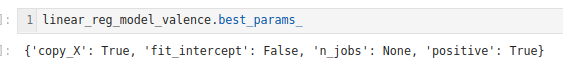
\includegraphics[width=0.7\linewidth]{figs/final_params_linear_valence}
		\caption{Hiperparámetros de la regresión lineal para la predicción de valencia}
		\label{fig:finalparamslinearvalence}
	\end{figure}
	\item Para activación:
	\begin{figure}[H]
		\centering
		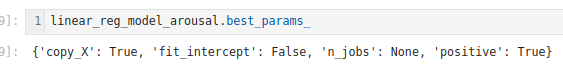
\includegraphics[width=0.7\linewidth]{figs/final_params_linear_arousal}
		\caption{Hiperparámetros de la regresión lineal para la predicción de activación}
		\label{fig:finalparamslineararousal}
	\end{figure}
\end{itemize}

Una vez obtenidos los hiperparámetros se construye el algoritmo de regresión lineal. Después se entrena el modelo con las variables de entrenamiento (\textit{X\_train\_val} y \textit{y\_train\_val} para valencia, y \textit{X\_train\_ar} y \textit{y\_train\_ar} para activación).


En este punto del experimento, el modelo de regresión lineal está listo para ser utilizado con los datos de test (\textit{X\_test\_val} y \textit{X\_test\_ar}). La precisión y la fiabilidad del modelo será evaluada en el capítulo \ref{resultados}.

\subsubsection{Regresión \textit{ridge}}
Para la implementación de los modelos de regresión \textit{ridge}, se ha utilizado la función \textit{Ridge}, perteneciente a la librería \textit{scikit-learn} de Python \cite{scikit-learn}.


Para el ajuste de hiperparámetros del modelo, se ha utilizado \textit{GridSearchCV} (función presente en el módulo \textit{model selection} de \textit{sckit-learn} \cite{scikit-learn}) para realizar una validación cruzada exhaustiva.

Uno de los parámetro de entrada de \textit{GridSearchCV} es \textit{param\_grid}. Este parámetro lee una selección de valores para cada hiperparámetro de \textit{LinearRegression}. Estos valores se recogen en la variable \textit{grid\_hp\_ridge\_reg} (Ver Figura \ref{fig:paramsridge}).
\begin{figure}[H]
	\centering
	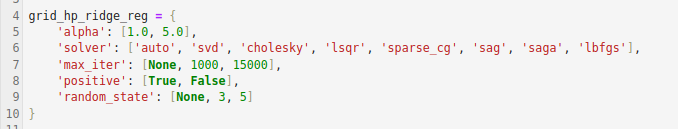
\includegraphics[width=0.7\linewidth]{figs/params_ridge}
	\caption{Variable \textit{grid\_hp\_ridge\_reg} para la validación cruzada de \textit{Ridge}}
	\label{fig:paramsridge}
\end{figure}


Los hiperparámetros elegidos por la validación cruzada para la regresión \textit{ridge} son:
\begin{itemize}
	\item Para valencia:
	\begin{figure}[H]
		\centering
		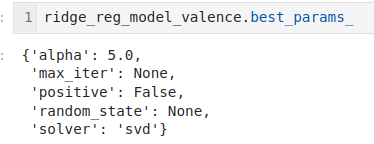
\includegraphics[width=0.5\linewidth]{figs/final_params_ridge_valence}
		\caption{Hiperparámetros de la regresión \textit{ridge} para la predicción de valencia}
		\label{fig:finalparamsridgevalence}
	\end{figure}
	\item Para activación:
	\begin{figure}[H]
		\centering
		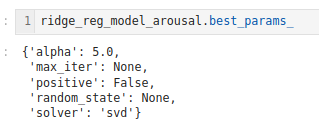
\includegraphics[width=0.5\linewidth]{figs/final_params_ridge_arousal}
		\caption{Hiperparámetros de la regresión \textit{ridge} para la predicción de activación}
		\label{fig:finalparamsridgearousal}
	\end{figure}
	
\end{itemize}

Una vez obtenidos los hiperparámetros se construye el algoritmo de regresión \textit{ridge}. Después se entrena el modelo con las variables de entrenamiento (\textit{X\_train\_val} y \textit{y\_train\_val} para valencia, y \textit{X\_train\_ar} y \textit{y\_train\_ar} para activación).


En este punto del experimento, el modelo de regresión \textit{ridge} está listo para ser utilizado con los datos de test (\textit{X\_test\_val} y \textit{X\_test\_ar}). La precisión y la fiabilidad del modelo será evaluada en el capítulo \ref{resultados}.









%%%%%%%%%%%%%% - RESULTADOS - %%%%%%%%%%%%%
\newpage
\section{Resultados}\label{resultados}
\subsection{Análisis de la características}
Para analizar los resultados obtenidos, primero se ha puesto el foco en las características. Mediante el uso de la función \textit{feature\_importances\_} se ha calculado la importancia que han tenido cada una de las variables independientes en los modelos de árbol de decisión y bosque aleatorio. Esta función devuelve un valor entre [0, 1], y la suma de todas las importancias de las características es igual a 1. Una vez calculadas todas las importancias, se han ordenado de mayor a menor para obtener una representación visual de las características más importantes.


En los modelos de árbol de decisión (tanto para la predicción de valencia como de activación), destacan muy pocas características por encima de la mayoría que tienen valor 0. En cada modelo, hay una característica que destaca por encima del resto (Figuras \ref{fig:importtreeregval} y \ref{fig:importtreeregar}): para valencia es \textit{audspec\_lengthL1norm\_sma\_de\_stddev}\footnote{Desviación estándar de los coeficientes delta de la media móvil suavizada de la norma L1 del espectro auditivo.}, y para activación \textit{audspec\_lengthL1norm\_sma\_amean}\footnote{Media aritmética de la media móvil suavizada de la norma L1 del espectro auditivo.}.
\begin{figure}[H]
	\centering
	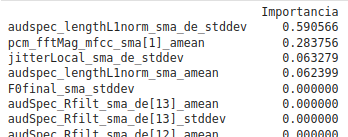
\includegraphics[width=0.6\linewidth]{figs/import_tree_reg_val}
	\caption{Características más importantes para árbol de decisión (predicción de valencia)}
	\label{fig:importtreeregval}
\end{figure}
\begin{figure}[H]
	\centering
	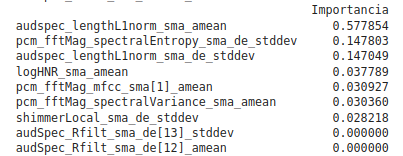
\includegraphics[width=0.7\linewidth]{figs/import_tree_reg_ar}
	\caption{Características más importantes para árbol de decisión (predicción de activación)}
	\label{fig:importtreeregar}
\end{figure}


Para los modelos de bosque aleatorio se observa un resultado similar al obtenido en los de árbol de decisión (Figuras \ref{fig:importrandomforestval} y \ref{fig:importrandomforestar}): unas pocas características tiene valor distinto de 0. En este caso los resultados están más suavizados, es decir, los valores de las características más importantes son similares. Destacan sobre el resto características diferentes en cada modelo: para el modelo de valencia destacan \textit{audspec\_lengthL1norm\_sma\_de\_stddev} y \textit{pcm\_fftMag\_mfcc\_sma[1]\_amean}\footnote{Media aritmética de los coeficientes cepstrales en la frecuencia Mel (MFCC) suavizados mediante una media móvil, calculados a partir de la magnitud de la FFT de la señal de audio digitalizada.}, y para activación \textit{audspec\_lengthL1norm\_sma\_amean}
\begin{figure}[H]
	\centering
	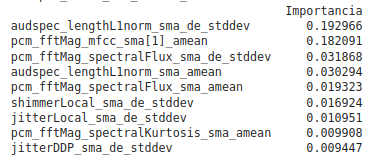
\includegraphics[width=0.7\linewidth]{figs/import_random_forest_val}
	\caption{Características más importantes para bosque aleatorio (predicción de valencia)}
	\label{fig:importrandomforestval}
\end{figure}
\begin{figure}[H]
	\centering
	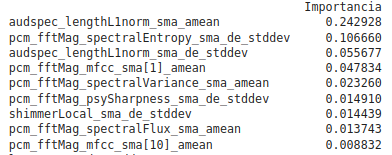
\includegraphics[width=0.7\linewidth]{figs/import_random_forest_ar}
	\caption{Características más importantes para bosque aleatorio (predicción de activación)}
	\label{fig:importrandomforestar}
\end{figure}


Para hacer el análisis en los modelos de regresión lineal y \textit{ridge} se ha empleado la función \textit{coef\_} para calcular los coeficientes de las variables independientes. Estos coeficientes representan la relación entre cada variable independiente con la variable dependiente. El rango de los coeficientes pueden ser cualquier número real, por lo que el rango es (-$\infty$, $\infty$):
\begin{itemize}
	\item Un coeficiente positivo indica una relación directa: a medida que la característica aumenta, el valor de la variable dependiente también tiende a aumentar.
	\item Un coeficiente negativo indica una relación inversa: a medida que la característica aumenta, el valor de la variable dependiente tiende a disminuir.
	\item Un coeficiente de 0 sugiere que la característica no tiene ninguna relación lineal con la variable dependiente.
\end{itemize}

Para regresión lineal (tanto en valencia como en activación) hay dos variables que destacan por encima del resto (Figuras \ref{fig:importlinearregval} y \ref{fig:importlinearregar}): \textit{shimmerLocal\_sma\_de\_amean}\footnote{Media aritmética de los coeficientes delta de la media móvil suavizada del shimmer local.} y \textit{jitterDDP\_sma\_de\_amean}\footnote{Media aritmética de los coeficientes delta de la media móvil suavizada del jitter DDP.}.
\begin{figure}[H]
	\centering
	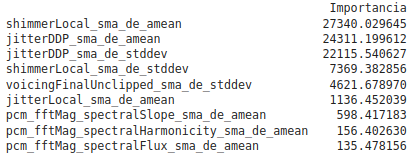
\includegraphics[width=0.7\linewidth]{figs/import_linear_reg_val}
	\caption{Características más importantes para regresión lineal (predicción de valencia)}
	\label{fig:importlinearregval}
\end{figure}
\begin{figure}[H]
	\centering
	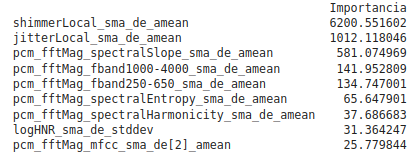
\includegraphics[width=0.7\linewidth]{figs/import_linear_reg_ar}
	\caption{Características más importantes para regresión lineal (predicción de activación)}
	\label{fig:importlinearregar}
\end{figure}
En los modelos de regresión \textit{ridge} no hay características que destaquen por encima del resto, y además, todos los valores están cercanos a 0 (Figuras \ref{fig:importridgeval} y \ref{fig:importridgear}). Esto indica que todas las características influyen de forma similar en el resultado de la variable objetivo.
\begin{figure}[H]
	\centering
	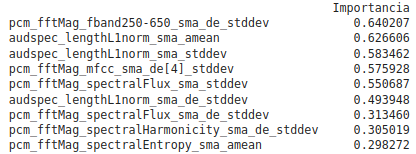
\includegraphics[width=0.7\linewidth]{figs/import_ridge_val}
	\caption{Características más importantes para regresión \textit{ridge} (predicción de valencia)}
	\label{fig:importridgeval}
\end{figure}
\begin{figure}[H]
	\centering
	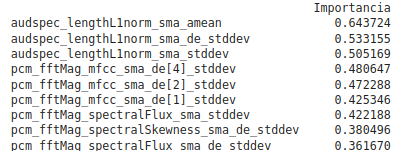
\includegraphics[width=0.7\linewidth]{figs/import_ridge_ar}
	\caption{Características más importantes para regresión \textit{ridge} (predicción de activación)}
	\label{fig:importridgear}
\end{figure}
	


\subsection{Comparativa de modelos}
La evaluación de modelos predictivos se realiza mediante la comparación de las variables objetivo (predichas por el sistema) con los valores reales. En este trabajo, al tener dos variables objetivo, han de compararse los resultados obtenidos para la valencia y para la activación por separado.

La salida de este sistema de MER es la predicción de emociones representadas por dos magnitudes. En decir, un punto en un espacio bidimensional. En la siguiente imagen \ref{fig:results} se muestra una comparativa entre el valor real y el predicho de cinco canciones del conjunto de variables de test. 
\begin{figure}[H]
	\centering
	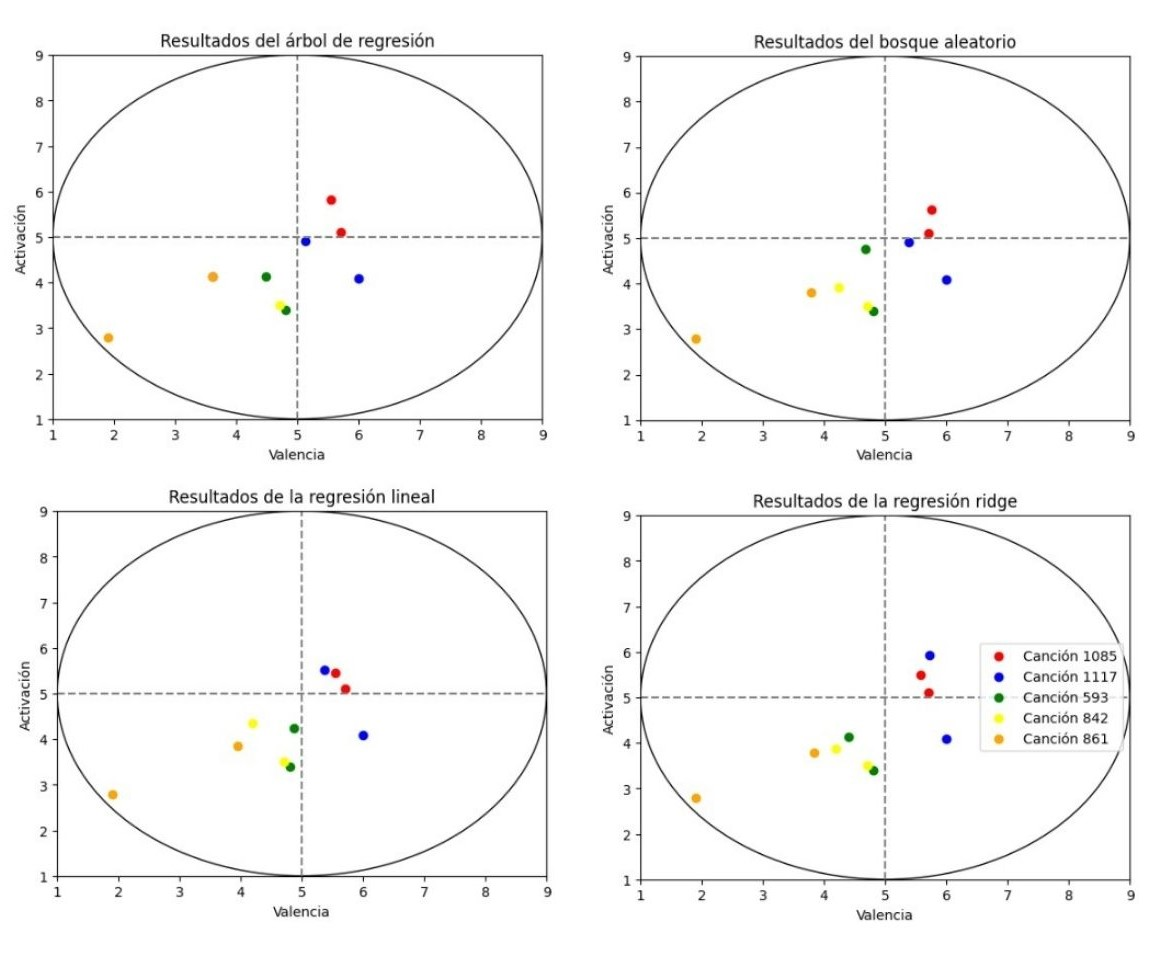
\includegraphics[width=1\linewidth]{figs/results}
	\caption{Comparativa de modelos}
	\label{fig:results}
\end{figure}


A simple vista, no es posible evaluar cómo de eficientes son los modelos empleados en el sistema. A diferencia de los problemas de clasificación (donde la precisión de los modelos se mide a partir de los fallos y aciertos del modelo), los modelos de regresión precisan de diferentes métricas para evaluar la efectividad. Los valores a predecir y los reales son continuos, y mediante las métricas de evaluación se mide lo cerca (o lejos) que están los datos reales de los predichos.
Las métricas elegidas para este experimento son:
\begin{itemize}
	\item \textit{Mean absolute error} (MAE)
	\item \textit{Mean squared error} (MSE)
	\item Coeficiente de determinación (R2 \textit{Score})
	\item \textit{Mean absolute percentage error} (MAPE)
\end{itemize}

Para obtener estas métricas se ha utilizado la librería de \textit{scikit-learn} de Python, y las funciones correspondientes para cada caso.

\subsubsection{Mean absolute error (MAE)}\label{mae}
El \textit{mean absolute error} (o error absoluto medio) se calcula como el promedio de las diferencias absolutas entre dos variables continuas. La fórmula del MAE es \cite{eswiki:146234007}:
\begin{equation}\label{eq:mae}
	MAE = \frac{1}{N} \sum_{i=1}^{N} |y_i - \hat{y}_i|
\end{equation}
donde
\begin{itemize}
	\item $N$ es el número de observaciones,
	\item $y_i$ es el valor real de la observación,
	\item $\hat{y}_i$ es el valor predicho.
\end{itemize}

Los resultados del MAE obtenidos durante el experimento son:
\begin{itemize}
	\item Para valencia:
	\begin{table}[H]
		\centering
		\caption{MAE de valencia}
		\label{tab:maevalencia}
		\begin{tabular}{|c|c|}
			\hline
			\textbf{Algoritmo} & \textbf{MAE} \\
			\hline
			Árbol de decisión & 0.811 \\
			Bosque aleatorio & 0.680 \\
			Regresión Lineal & 0.649 \\
			Regresión \textit{ridge} & 0.696 \\
			\hline
		\end{tabular}
	\end{table}
	\item Para activación:
	\begin{table}[H]
		\centering
		\caption{MAE de activación}
		\label{tab:maeactivacion}
		\begin{tabular}{|c|c|}
			\hline
			\textbf{Algoritmo} & \textbf{MAE} \\
			\hline
			Árbol de decisión & 0.842 \\
			Bosque aleatorio & 0.718 \\
			Regresión Lineal & 0.795 \\
			Regresión \textit{ridge} & 0.852 \\
			\hline
		\end{tabular}
	\end{table}
\end{itemize}

Si se observa la fórmula \eqref{eq:mae}, MAE mide la diferencia media entre el valor real y el valor predicho. Por lo tanto, el mejor modelo respecto a esta métrica será aquel con el menor MAE. En las tablas \ref{tab:maevalencia} y \ref{tab:maeactivacion} se puede ver que los modelos con mejor puntuación son: regresión lineal para valencia, y bosque aleatorio para activación.


La interpretación del MAE se hace en función de los valores posibles de la variable dependiente, que para este caso, tanto valencia como activación están entre 1 y 9 (esta relación se puede ver mejor en el apartado \ref{mape} donde se analiza la métrica MAPE). Observando los resultados, los modelos con mejor puntuación MAE predicen con un error de 0.649 y 0.718 respectivamente.



\subsubsection{Mean squared error (MSE)}
El \textit{mean squared error} (o error cuadrático medio) es similar al MAE, con la diferencia de que mide el promedio de los errores al cuadrado. La fórmula del MSE es \cite{eswiki:159951880}:
\begin{equation}
	MSE = \frac{1}{N} \sum_{i=1}^{N} (y_i - \hat{y}_i)^{2}
\end{equation}
donde
\begin{itemize}
	\item $N$ es el número de observaciones,
	\item $y_i$ es el valor real de la observación,
	\item $\hat{y}_i$ es el valor predictivo.
\end{itemize}

Los resultados del MSE obtenidos son:
\begin{itemize}
	\item Para valencia:
	\begin{table}[H]
		\centering
		\caption{MSE de valencia}
		\label{tab:msevalencia}
		\begin{tabular}{|c|c|}
			\hline
			\textbf{Algoritmo} & \textbf{MSE} \\
			\hline
			Árbol de decisión & 0.904 \\
			Bosque aleatorio & 0.688 \\
			Regresión Lineal & 0.646 \\
			Regresión \textit{ridge} & 0.708 \\
			\hline
		\end{tabular}
	\end{table}
	\item Para activación:
	\begin{table}[H]
		\centering
		\caption{MSE de activación}
		\label{tab:mseactivacion}
		\begin{tabular}{|c|c|}
			\hline
			\textbf{Algoritmo} & \textbf{MSE} \\
			\hline
			Árbol de decisión & 1.035 \\
			Bosque aleatorio & 0.806 \\
			Regresión Lineal & 0.946 \\
			Regresión \textit{ridge} & 1.094 \\
			\hline
		\end{tabular}
	\end{table}
\end{itemize}

Al igual que MAE, cuanto menor sea el valor obtenido, mejor será el modelo. Los resultado obtenidos de esta métrica son (ver tablas \ref{tab:msevalencia} y \ref{tab:mseactivacion}): modelo de regresión lineal para valencia con una MSE de 0.646, y modelo de bosque aleatorio para activación con un valor de 0.806. Ambos valores son menores que 1, por lo que el resultado para los modelos se puede considerar bueno. 

\subsubsection{Coeficiente de determinación (R2 \textit{score})}
El coeficiente de determinación (R2 \textit{score}) mide la varianza en la variable objetivo a partir de las variables independientes. Su fórmula es \cite{eswiki:158364923}:
\begin{equation}
	R2 = 1 - \frac{\sigma^{2}_r}{\sigma^{2}_y} 
\end{equation}
donde
\begin{itemize}
	\item $\sigma^{2}_r$ es la varianza de la variable residual (diferencia entre lo real y lo predicho),
	\item $\sigma^{2}_y$ es la varianza de la variable independiente.
\end{itemize}

Los valores obtenidos son los siguientes:
\begin{itemize}
	\item Para valencia:
	\begin{table}[H]
		\centering
		\caption{Coeficiente R2 para valencia}
		\label{tab:r2valencia}
		\begin{tabular}{|c|c|}
			\hline
			\textbf{Algoritmo} & \textbf{R2} \\
			\hline
			Árbol de decisión & 0.303 \\
			Bosque aleatorio & 0.469 \\
			Regresión Lineal & 0.502 \\
			Regresión \textit{ridge} & 0.454 \\
			\hline
		\end{tabular}
	\end{table}
	\item Para activación:
	\begin{table}[H]
		\centering
		\caption{Coeficiente R2 para activación}
		\label{tab:r2activacion}
		\begin{tabular}{|c|c|}
			\hline
			\textbf{Algoritmo} & \textbf{R2} \\
			\hline
			Árbol de decisión & 0.363 \\
			Bosque aleatorio & 0.504 \\
			Regresión Lineal & 0.417 \\
			Regresión \textit{ridge} & 0.326 \\
			\hline
		\end{tabular}
	\end{table}
\end{itemize}

Los valores de R2 varían entre 0 y 1 (aunque hay casos donde puede ser negativo si el modelos es muy inadecuado). Si $R2 = 1$ significa que el modelo explica toda la variabilidad de la variable independiente, mientras que si $R2 = 0$ no lo hace. En los resultados (tablas \ref{tab:r2valencia} y \ref{tab:r2activacion}) se observa que los modelos con mejor R2 son: regresión lineal para valencia, y bosque aleatorio para activación. Ambos valores están alrededor de 0.5, lo que quiere decir que los modelos explican el 50\% de la variabilidad de los datos. Para un caso como el que presenta este trabajo donde hay muchas variables independientes, se puede decir que el valor de R2 conseguido es generalmente bueno.

\subsubsection{Mean absolute percentage error (MAPE)}\label{mape}
El \textit{mean absolute percentage error} (error porcentual absoluto medio) mide la precisión de la predicción como una proporción entre el valor real y el valor predicho. Su fórmula es \cite{enwiki:1225070385}:
\begin{equation}
	MAPE = 100 \frac{1}{N} \sum_{t=1}^{N} |\frac{A_t - F_t}{A_t}|
\end{equation}
donde
\begin{itemize}
	\item $N$ es el número de observaciones,
	\item $A_t$ es el valor real,
	\item $F_t$ es el valor predicho.
\end{itemize}

Los resultados obtenidos del MAPE son:
\begin{itemize}
	\item Para valencia:
	\begin{table}[H]
		\centering
		\caption{MAPE de valencia}
		\label{tab:mapevalencia}
		\begin{tabular}{|c|c|}
			\hline
			\textbf{Algoritmo} & \textbf{MAPE} \\
			\hline
			Árbol de decisión & 0.170 \\
			Bosque aleatorio & 0.143 \\
			Regresión Lineal & 0.137 \\
			Regresión \textit{ridge} & 0.149 \\
			\hline
		\end{tabular}
	\end{table}
	\item Para activación:
	\begin{table}[H]
		\centering
		\caption{MAPE de activación}
		\label{tab:mapeactivacion}
		\begin{tabular}{|c|c|}
			\hline
			\textbf{Algoritmo} & \textbf{MAPE} \\
			\hline
			Árbol de decisión & 0.181 \\
			Bosque aleatorio & 0.160 \\
			Regresión Lineal & 0.174 \\
			Regresión \textit{ridge} & 0.186 \\
			\hline
		\end{tabular}
	\end{table}
\end{itemize}

Esta métrica es similar a MAE (ver apartado \ref{mae}), con la diferencia de que representa el error en forma de porcentaje. Los modelos con menor porcentaje de error son los modelos más precisos. Según los resultados observados en el experimento (ver tablas \ref{tab:mapevalencia} y \ref{tab:mapeactivacion}), los modelos más precisos son: regresión lineal para valencia, con un 13.7\% de error; y bosque aleatorio para activación con 16\% de error. En general, los modelos pueden considerarse como buenos según esta métrica. 










%%%%%%%%%%%%%% - CONCLUSIONES - %%%%%%%%%%%%%
\newpage
\section{Conclusiones}
En este trabajo se ha realizado una comparativa de algoritmos de regresión para la predicción de emociones musicales. Para ello se ha realizado un estudio previo de la disciplina de MER (marco teórico, estado actual y futuro). También se han definido los problemas de regresión de \textit{Machine Learning} y las técnicas empleadas en el experimento. Finalmente, se han aplicado los distintos modelos y se han calculado métricas para valorar su rendimiento.


A continuación se detallan las conclusiones obtenidas de los resultados del experimento. Se analizan también las competencias adquiridas durante el estudio del Grado que fueron empleadas en el trabajo. Por último, se proponen las posibles líneas futuras que seguiría el trabajo.

 
\subsection{Conclusiones}
El primer objetivo propuesto para el trabajo es el estudio de la disciplina de MER. Este objetivo se ha cumplido: para la elaboración del capítulo de \textit{Estado del arte} se ha llevado a cabo una investigación sobre este campo mediante la lectura de libros, artículos y trabajos.


La primera conclusión obtenida del trabajo, es la complejidad del campo de estudio de MER. Partiendo de la propia naturaleza de las emociones, no es posible construir un sistema que prediga la totalidad de las emociones que un oyente extrae de la escucha de una canción. El apartado \ref{emo} describe dos tipos de emociones (percibidas e inducidas). Mediante el análisis de las características acústicas de la canción solo se pueden estimar las emociones percibidas, al estar relacionadas directamente con el momento de la escucha de la canción. Un sistema en el que se introduzcan variables o elementos que analicen las emociones inducidas sería demasiado complejo.


Los experimentos se han desarrollado en su totalidad usando el lenguaje Python, cumpliendo así los objetivos marcados para el trabajo. El uso de los cuadernos Jupyter ha resultado de gran ayuda para la ejecución del código. Al igual que las librerías como \textit{scikit-learn} o \textit{Pandas}, muy útiles para el desarrollo de algoritmos y el manejo de datos.


Desde el punto de vista del empleo de técnicas de \textit{Machine Learning} se concluye que, los modelos óptimos no son los mismos para predecir valencia que para predecir activación. Los resultado son claros: todas las métricas utilizadas para la comparativa han dado los mismo resultados. En el caso de valencia, el algoritmo óptimo es la regresión lineal. Mientras que para activación es el bosque aleatorio.  Al ser un sistema compuesto por dos variables objetivo diferente, se puede usar un algoritmo diferente para cada una.




\subsection{Competencias y conocimientos}
En el desarrollo del trabajo, se han empleado diferentes técnicas y conocimientos adquiridos durante el estudio del Grado. Algunas de ellas son:
\begin{itemize}
	\item Uso del lenguaje Python de programación. Conocimiento adquirido a través del estudio de varias asignaturas como \textit{Protocolos para la Transmisión de Audio y Video en Internet} o \textit{Tratamiento Digital del Sonido}. Más específicamente, el uso del entorno de Anaconda y los cuadernos Jupyter. El uso de este entorno para desarrollos de \textit{Machine Learning} es bastante habitual, motivo de su elección para el desarrollo del experimento.
	\item De la asignatura de \textit{Tratamiento Digital del Sonido} también se han adquirido los conocimientos necesarios para el uso y el manejo de las características acústicas de las canciones.
	\item Durante el experimento, se emplean técnicas de \textit{Machine Learning}. En la asignatura de \textit{Tratamiento Digital del Sonido} se aprendieron los conocimientos básicos de este campo, y algunas de las técnicas empleadas durante el trabajo.
	\item De la asignatura \textit{Estadística para Medios Audiovisuales}, se adquirieron los conocimientos para comprender los conceptos estadísticos de las métricas utilizadas en la evaluación de los modelos.
\end{itemize}

Además de las competencias adquiridas durante el estudio del Grado, otras nuevas se han aprendido en el desarrollo del trabajo. Como son:
\begin{itemize}
	\item Empleo del lenguaje Latex para la redacción de la memoria. Su uso ha resultado de gran ayuda para estructurar el texto, o incluir en la composición de la memoria diferentes elementos como referencias, imágenes y tablas.
	\item Aumentar el conocimiento en \textit{Machine Learning} mediante técnicas y algoritmos no estudiados en el Grado.
	\item Conocimiento adquirido durante la investigación en el campo de estudio de MER.
\end{itemize}
\subsection{Futuras líneas de trabajo}

Una vez realizados los experimentos propuestos para el trabajo se detectan las siguientes líneas de estudio futuras para continuar mejorando y expandiendo esta aplicación MER:
\begin{itemize}
	\item Implementación de otros algoritmos y técnicas de \textit{Machine Learning} con el objetivo de mejorar las puntuaciones de precisión en la predicción obtenidas en el experimento.
	\item Hubiera sido interesante contar con una base de datos donde, el espacio bidimensional de Russell, estuviera segmentado en distintas emociones. Como se comentaba en el apartado \ref{combi}, una combinación discreta-dimensional de la taxonomía de las emociones puede ayudar en la efectividad del modelo. De esta forma, la aplicación sería mucho más intuitiva puesto que trabajaría directamente con emociones discretas en lugar de su representación mediante valencia-activación. Por ejemplo, si una canción está identificada con la emoción ``alegre'', se puede probar a simple vista si la aplicación predijo ``alegre'' de forma satisfactoria u otra emoción.
	\item La letra de las canciones juega un papel importante en las emociones percibidas por el oyente. Una posible línea de trabajo es la introducción de la letra como una variable independiente más del modelo. Al estudiar solo las características acústicas de la canción, se pierden los posibles matices que pueda tener la letra. Una canción puede tener una letra triste pero sin embargo una música alegre, entonces la emoción percibida se puede ver ``contaminada'' en gran manera por la letra.
	\item El complemento más obvio a este trabajo es la integración de este desarrollo en una aplicación final (de interfaz de usuario amigable). Un caso claro sería un reproductor streaming de música, que pueda recomendar o clasificar canciones en función de sus emociones. O un editor de video que, como complemento a la imagen, quiera incluir música específica para evocar en el usuario una emoción precisa.
\end{itemize}





%%%%%%%%%%%%%% - BIBLIOGRAFÍA - %%%%%%%%%%%%%
\newpage
\section{Bibliografía}
\printbibliography[heading=none]

\end{document}
